\chapter{The search for absolute velocity}

\index{search for absolute velocity}
%%%%%%%%%%%%%%%

\newpage

\thispagestyle{empty}
\begin{figure}[H]
\centering
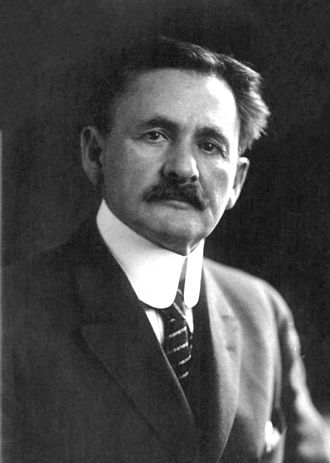
\includegraphics[scale=.5]{src/images/lbk-graphics/portraits/michelson-wiki.jpg}
\caption*{Albert Abraham Michelson}
\end{figure}
%~ \portrait{1}{lbk-graphics/portraits/michelson-wiki.jpg}%
%~ {Albert Abraham Michelson}
\begin{small}
\begin{quote}
Albert Abraham Michelson (December 19, 1852 -- May 9, 1931) 
was an American physicist known for his work on the 
measurement of the speed of light and especially for the 
Michelson-Morley experiment. In 1907 he received the Nobel 
Prize in Physics. He became the first American to receive 
the Nobel Prize in sciences.
\hfill --Wikipaedia
\end{quote}
\end{small}
\newpage


\section{Introduction}

In this section, to present the discussion in the proper 
historical perspective, we accept, tentatively, the 
Newtonian postulate that space is Euclidean and absolute. 
Then,  we introduce a global Cartesian coordinate system  
at rest relative to  absolute space, call it the absolute 
frame \index{absolute  !  frame} and agree to follow the 
Newtonian convention that all motion shall be reckoned 
against the absolute frame only.  We may recall that the 
Newton laws of motion pertain to {absolute motion}, (i.e., 
motion relative to the absolute frame) only. Obviously, the 
absolute frame, \textsl{if it exists}, would provide a  
universal preferred standard of rest\footnote{Wolfgang  
Rindler, loc.cit.}. If one could some how measure the 
absolute velocity \index{absolute !  velocity} $\vec{v}$ of 
an object, (i.e., its velocity relative to the absolute 
frame), one would have identified the absolute frame 
relative to which the particle has that velocity $\vec{v}$. 
This way, by determining the absolute velocity of an object, 
one would identify the absolute frame and hence the  
absolute space postulated by Newton.\index{absolute ! space}

This idea motivated the great \textsl{search for 
absolute velocity} \index{search for absolute velocity} in 
the nineteenth century. However, it had been  realised 
that the Newton laws of motion, and the Newton law of 
universal gravitation were both Galilei-invariant and hence 
would  not help in marking out the absolute frame 
from among the class of all Gali\-lean frames. Therefore one 
had to look beyond these  Newtonian laws for identifying 
the absolute frame. The notion of the absolute space (and 
hence that of the absolute frame) had been introduced by 
Newton, and physicists who had great faith in the genius of 
Newton, fondly believed that absolute frame exists and hoped 
that some one would discover a way of identifying it 
experimentally. But much against their hope, for almost two 
hundred years, no experimental method of identifying the 
absolute frame was discovered. Then, towards the end if the 
nineteenth century, there emerged a ray of hope.

The electromagnetic theory of Maxwell, available as a 
`well-finished' physical theory by the year 1873, predicted 
physical phenomena which could distinguish between the 
absolute frame and the other Galilean frames. In its 
original formulation, the electromagnetic theory of Maxwell 
postulated that the electromagnetic fields are (mechanical) 
excitations of a material medium called {luminiferous 
ether}\index{luminiferous ether}. Further, the Maxwell 
theory said that this ether medium  is present everywhere in 
the universe, even inside matter, and is at rest relative to 
the absolute frame, i.e., the ether mediumin a state of 
absolute rest\index{state of absolute rest}. It also 
identified light as an electromagnetic wave in ether, 
postulated that the ether medium is isotropic and 
non-dispersive for the propagation of light. 

Maxwell's  theory had predicterd that the absolute speed 
of electromagnetic waves in ether (denoted by the symbol 
$c$), could also be determined as the ratio of the 
capacitances of a condenser in the electromagnetic (emu) and 
electrostatic (esu) system of units. \index{absolute speed 
of electromagnetic  waves in ether} In 1856, Weber and 
Kohlrauch\footnote{W.Weber and R.Kohlrauch, {Ann. der 
Phys}., {99}, 10, 1856.} determined this ratio 
experimentally. Very surprisingly, this ratio of 
capacitances coincided with the speed of light determined 
earlier by Roemer and others.  Maxwell could see the 
significance of this coincidence and he correctly 
conjectured that light is an electromagnetic wave. 

Here, in the following paragraphs, for convenience, let us 
call a frame obtained by a Galileo-transformation from the 
absolute frame, a \textsl{moving Galilean frame}. 
\index{moving Galilean frame}Then, if $\vec{u}$, is the 
velocity of light in the absolute frame \index{velocity of 
light in the absolute frame}(that is, its absolute 
velocity), its velocity $\pvec{u}$ relative to any other 
moving Galilean frame $S'$ would be
\begin{align}\label{sav.1}
\pvec{u}=\vec{u}-\vec{v}.
\end{align}
Taking the ``dot'' product of this relation with a given 
unit vector $\uvec{n}$, we get the relation between speeds 
of light in the two frames in the spatial 
direction $\uvec{n}$:
\begin{align*}
c'_n=c-v_n,
\end{align*}
where we have written  $c'_n\equiv \pvec{u}\dotp \uvec{n}$,
$\vec{u}\dotp \uvec{n} = c$ and $v_n\equiv \vec{v}\dotp 
\uvec{n}$. This formula shows that, with the exception of 
the absolute frame, in all other moving Galilean frames, 
light would propagate with (slightly) different speeds 
$c'_n$ in different spatial directions specified by 
$\uvec{n}$. 
\begin{quote}
\textsl{Thus, the absolute frame would be that unique frame 
in which light propagates isotropically in ether.}          
\end{quote}

This conclusion could be experimentally tested and at last, 
one knew exactly how to identify the absolute frame. Only a 
suitable experiment (although difficult in view of the 
unusually large vacuum velocity of light) had to be designed 
to test this Maxwellian prediction and once that was done, 
the long search for the absolute space would be over!

\vspace{-.2cm}

\section{The Michelson-Morley experiment}
An experiment to test if the speed of light was dependent 
on the direction of propagation of light in a moving 
Galilean frame was done by Michelson in 1881. Michelson 
repeated this experiment with the collaboration of Morley 
in Germany in the following years 1882-1887.  

\begin{quote}
\textsl{The essential idea of the experiment was to compare 
the `up'' and `down' trip-times of light along two paths in 
mutually perpendicular directions. One of the two 
perpendicular directions was chosen along the direction of 
the orbital velocity of the earth round the sun.}
\end{quote}

A precision optical instrument to measure the minute  
difference in the trip-times along two mutually 
perpendicular paths, known as the Michelson interferometer  
today, was designed by  Michelson and used in this 
experiment. The schematics of the experimental set-up is 
shown in \figref{fig3.1}. 

\newpage

\begin{figure}[H]
\centering
\begin{tikzpicture}
%   \draw[help lines,step=.25,brown] (-5,-5) grid (5,5) ;
%   \foreach \y in {-4.5,-4,...,4.5,}
%     \draw (-5.2,\y) node[left]{\small \y} ;
%     \foreach \y in {-5,-4.5,...,4,4.5}
%     \draw (5.2,\y) node[right]{\small \y} ;  
%   \foreach \x in {-4.5,-4,...,5}
%     \draw (\x,5.15) node{\small \x} ;
%  \foreach \x in {-5,-4,...,5}
%  \draw (\x,-5) node[below]{\small \x} ; 
 \node at (0,0){\ingr{.6}{src/images/lbk-graphics/mm-new.pdf}};
  \node at (-.95,-3.2){\small $T$} ;
\node at (-.7,-1.25){\small  $O$} ;
\node at (3.3,-1){\small  $M_1$} ;
\node at (-.88,3.1){\small  $M_2$} ;
\node at (-3.2,-1){\small  $P$} ;
\node at (-1.6,-1.6){\small  $G_1$} ;
\node at (.5,-1.6){\small  $G_2$} ;
\node at (1.5,-1.25){$d$} ;
\node at (-.75,1){$d$} ;
\end{tikzpicture}
\caption{Schematics of the Michelson-Morley experiment} 
\label{fig3.1}
\end{figure}

First we describe, briefly, the essential Michelson 
interferometer. The instrument consists of a monochromatic 
light-source $P$, two optically flat glass plates $G_1$ and 
$G_2$, a pair of  flat front-silvered mirrors $M_1$ and 
$M_2$ and a telescope $T$ arranged as shown in 
\figref{fig3.1}. The positions of $G_1$,  $G_2$ (except for 
a provision for a small adjustment of its tilt), $M_1$ and 
$M_2$ are all fixed rigidly to the heavy base of the 
interferometer.  

Light from $P$ falling on $M_1$ gets split into two beams of 
rough\-ly equal intensities travelling in perpendicular 
directions. For convenience, we may label these beams as 
beam-1 and beam-2.  One of the beams, which we have labelled 
as  beam-2, is reflected upwards at $G_1$, falls on a flat 
front-silvered mirror $M_2$, gets reflected down, passes 
through $G_1$ again and eventually reaches the telescope 
$T$. The other beam, namely beam-1, passes through $G_1$ and 
then through another glass plate\footnote{The plate $G_2$, 
called a compensating plate, is used for introducing a 
small, path-difference (between the beams 1 and 2) which is 
over and above that  introduced by the difference in light 
speeds in the directions of the beams 1 and 2.}
\footnote{The plate $G_2$ is identical to $G_1$ and kept 
approximately parallel to $G_1$.} $G_2$,  suffers normal 
reflection at the front-silvered mirror $M_1$, retraces its 
path and reaches the telescope $T$ after getting reflected 
at $G_1$ again. When conditions for interference are 
favourable,  beams 1 and 2  travelling towards $T$ 
interefere and intereference patterns are observed in the 
focal plane of the telescope $T$.

We need to calculate the difference in the time taken by 
light for the two trips $G\rightarrow M_1\rightarrow G$ and 
and $G\rightarrow  M_2\rightarrow G$: We denote the time 
taken by light for the former trip by the symbol 
$t_\parallel$ and the latter trip by the symbol $t_\perp$. 
The difference $\gkd t\equiv t_\parallel-t_\perp$ may be 
calculated either in the absolute frame $S$ in which ether 
is at rest while the earth is in motion, or,  in the moving 
earth-bound frame $S'$ in which the earth (along with the 
laboratory and the Michelson interferometer) is at rest. We 
do the calculation in both the frames below:

\vspace{-.2cm}

\subsection{Calculation of {$\gkd t$} in 
the absolute frame}
\begin{figure}[H]
\centering
\begin{tikzpicture}
%   \draw[help lines,step=.25,brown] (-5,-5) grid (5,5) ;
%   \foreach \y in {-4.5,-4,...,4.5,}
%     \draw (-5.2,\y) node[left]{\small \y} ;
%     \foreach \y in {-5,-4.5,...,4,4.5}
%     \draw (5.2,\y) node[right]{\small \y} ;  
%   \foreach \x in {-4.5,-4,...,5}
%     \draw (\x,5.15) node{\small \x} ;
%  \foreach \x in {-5,-4,...,5}
%  \draw (\x,-5) node[below]{\small \x} ; 
 \node at 
(.2,.32){\ingr{1.4}{src/images/lbk-graphics/orbit1-new.pdf}};
  \node at (0.7,-3){\small $T$} ;
 \node at (2,.57){\small  $v$} ;
 \node at (2.4,-1.75){\small  $M_1$} ;
  \node at (3.75,-1.75){\small  $M'_1$} ;
  \node at (-3.5,-1.75){\small  $P$} ; 
  \node at (5,-1.5){\small  $x,x'$} ;
  
\node at (-.75,-1.75){\small  $Q$} ;
\node at (-2,-1.75){\small  $G_1$} ;
\node at (1,-1.75){\small  $G'_1$} ;
\node at (-2.15,3.75){\small  $y$} ;
\node at (-.72,3.82){\small  $y'$} ;
\node at (-3.15,2.75){\small  $M_2$} ;
\node at (.29,2.75){\small  $M'_2$} ;
\end{tikzpicture}
\caption{} 
\label{fig3.2}
\end{figure}

\textsl{In the absolute frame in which ether is at rest, 
light travels with the \textsl{same} speed, say $c$,  in all 
the spatial directions}. Also, the Michelson interferometer 
\index{Michelson interferometer} which is attached to the 
earth is transported by the earth with the speed $v$ in its 
motion round the sun. We assume that one of  the arms of the 
Michelson interferometer, which carries the mirror $M_1$, is 
oriented along the positive $x$-axis while the other arm 
which carries the mirror $M_2$, has been oriented along the 
positive $y$-axis (\figref{fig3.2}). Further, we assume that 
the positive $x$-axis of the frame has been chosen to be 
along the instantaneous orbital velocity $\vec{v}$ of the 
earth round the sun. In \figref{fig3.2}, $\{G_1$, $M_1$, 
$M_2\}$, and $\{G'_1$, $M'_1$, $M'_2\}$ correspond 
respectively to two instantaneous positions of these objects 
(fixed to the moving interferometer) at the initial instant 
at which light leaves $G_1$ and at the later instant at 
which it is reflected (simultaneously) from $M'_1$ and 
$M'_2$.

\hsl{(i)~The light-trip $G_1 \rightarrow M'_2\rightarrow 
G'_1$} With reference to \figref{fig3.2}, let the 
interferometer be set such that the distances $GM_1 = 
GM_2=d$. As the mirror $M_2$ (fixed to the Michelson 
interferometer) moves in ether (with the velocity 
$\vec{v}=v\,\eye$), only light which travels along a slanted 
path (namely $GM_2'$ in \figref{fig3.2}) reaches $M_2$. The 
time taken by light for the trip $G\rightarrow M'_2$ is 
obviously $t =G M_2'/c$.  Also, in this time $t$,  $M_2$ 
which moves with a speed $v$,  would travel a distance $M_2 
M_2' =GQ=vt$. Then (see \figref{fig3.2}), $c^2 t^2$ 
$=GM_2^{'2}= GQ^2 + QM_2^{'2}=v^2 t^2+d^2$ so that
\begin{align*}
t =\frac{d/c}{\sqrt{1-\beta^2}}\quad\text{ where } 
\beta\equiv \frac{v}{c}. 
\end{align*} 
By symmetry (\figref{fig3.2}), the time taken for the 
return trip $M'_2\rightarrow G'$ is also equal to the $t$ 
calculated above. Hence, the total trip-time for light on 
the path $G\rightarrow  M'_2\rightarrow G'$ is
\begin{align}\label{sav.2}
t + t =\frac{2d/c}{\sqrt{1-\beta^2}}\equiv t_\perp.
\end{align}

\hsl{(ii)~The light-trip $G_1 \rightarrow M'_1$} With 
reference to \figref{fig3.2}, let $t'$ be time taken by 
light to travel from $G_1$ to $M'_1$. In this time-interval 
$t'$, the mirror $M_1$ moves away from $G_1$ to the position 
$M'_1$ with the distance $M_1M_1'=vt'$.  Thus, light travels 
a total distance of $d'=GM_1+ M_1M'_1=d+vt'$to arrive at 
$M'_1$. The time taken by light for this trip is $(d+vt')/c$ 
which must clearly be the same as $t'$. Thus, $(d+vt')/c=t'$ 
which gives $t'=(d/c)/(1-v/c)$. 

\hsl{(iii)~The light-trip $M'_1 \rightarrow G'_1$} Again, 
with reference to \figref{fig3.2}, we now consider the trip 
pf light which leaves $G_1$, arrives at the new position 
$M'_1$ of the mirror $M_1$, gets reflected (instantaneously) 
and meets the glass plate $G_1$ at its new position $G'_1$. 
Suppose, the time taken by light to travel from $M'_1$ to  
$G'_1$ is $t''$. In this time-interval $t''$, the mirror 
$M_1$ must have travelled a distance of $M_1 M_1' =vt''$ 
\textsl{towards} $G_1$. Thus, in the trip $M'_1 \rightarrow 
G'_1$ light travels a distance $d'=GM_1-M_1M'_1=d-vt'$. The 
time taken for this trip is clearly $(d-vt'')/c$ which must 
be the same as $t''$. Thus, we have $t''=(d-vt'')/c$ which 
yields $t''=(d/c)/(1+v/c)$. Hence, the total time taken by 
light for the trip $G\rightarrow  M'_1\rightarrow G$, is
\begin{align}\label{sav.3}
 t' + t''  = \frac{(d/c)}{1-\gkb}+  
\frac{(d/c)}{1+\gkb} = \frac{(2d/c)}{1-\beta^2}\equiv 
t_\parallel.
\end{align}
The difference in the trip-times given in 
Eqns. \eqref{sav.2} and \eqref{sav.3} is
\begin{align}\label{sav.4} 
\delta t= t_\parallel -t_\perp =
\frac{2d}{c}\left\{\frac{1}{1-\beta^2}
-\frac {1} { \sqrt {1-\beta^2}}\right\}\notag \\
\approx
\frac{2d}{c}\left\{1+\beta^2-(1+\frac{1}{2}\beta^2)\right\}
=(d/c) \beta^2.
\end{align}
This time difference corresponds to a path-difference 
$\delta =c \delta t$ between the two beams (light-waqves) 
arriving at the telescope. If an interference  
pattern has already been set up in the Michelson 
interferometer by introducing an initial path-difference 
$\delta_0$ (which can be done by adjusting the screws on 
the mirror-mounts of the Michelson interferometer), the 
path-difference $\delta$ (due to the difference in the 
light speeds) adds up with $\delta_0$ to produce a total 
path-difference $\delta_0+ \delta$. In the focal plane of 
the telescope, one should now see an interference pattern 
due to the total path-difference $\delta_0+ \delta$. There 
is no way in which $\delta$ can be separated from 
$\delta_0$ and it appears that $\delta_0$ is undetectable. 
However, if we now rotate the Michelson interferometer, en 
bloc, from this configuration, through $\pi/2$ in the 
clockwise direction (In the experiment of Michelson, the 
heavy base of the Michelson interferometer floated on a pool 
of mercury and it could be rotated easily as required.),  
the mirror $M_2$ comes on to the positive $x$-axis while the 
other mirror $M_1$ moves down to the negative $y$-axis. It 
is easy to see that the total path-difference would then be 
$\delta_0-\delta$. Thus, the net path-difference introduced
between the two beams after the $\pi/2$ rotation of the 
Michelson interferometer would be
\begin{align}]\label{sav.5}
&\delta_0+\delta -(\delta_0-\delta) = 2\delta 
\notag\\&=2c\,\delta t
\approx (2d) \beta^2 \approx 2d\SI{e-8}{m},
\end{align}
where we have assumed  typical  values $v\sim\SI{3e4}{m. 
s^{-1} }$ and $c =\SI{3e8}{m.s^{-1}}$. Since one wavelength 
$ \lambda$ of path-difference corresponds to one 
fringe-shift, the above path-difference leads to a 
fractional fringe-shift of
\begin{align}\label{sav.6}
\sigma \approx (2d/\lambda) .10^{-8}.
\end{align}
In the original apparatus of Michelson, $d$ was 
$\SI{1.2}{m}$ and the wavelength $ \lambda$ was $ 
\sim\SI{600 e-9} {m}$, so that
\begin{align}\label{sav.7}
\sigma\approx  0.04.
\end{align}
\begin{quote}
\textsl{Although, the apparatus of Michelson could well 
have detected a fractional fringe shift of this magnitude, 
no significant fringe shift was detected by Michelson.}
\end{quote}

\subsection{Calculation of {$\gkd t$} in 
an earth-bound frame}
As remarked earlier, it is instructive to calculate $\gkd t$ 
in an earth-bound frame. We do that now:
\begin{figure}[H]
\centering
\begin{tikzpicture}
%   \draw[help lines,step=.25,brown] (-5,-5) grid (5,5) ;
%   \foreach \y in {-4.5,-4,...,4.5,}
%     \draw (-5.2,\y) node[left]{\small \y} ;
%     \foreach \y in {-5,-4.5,...,4,4.5}
%     \draw (5.2,\y) node[right]{\small \y} ;  
%   \foreach \x in {-4.5,-4,...,5}
%     \draw (\x,5.15) node{\small \x} ;
%  \foreach \x in {-5,-4,...,5}
%  \draw (\x,-5) node[below]{\small \x} ;
\node at (0,0){\ingr{.6}{src/images/lbk-graphics/orbit2a.pdf}};
 \node at (2.3,1.65){\small  $x, x'$} ;
 \node at (-2.2,2.4){\small  $y,y'$} ;
 \node at (0.2,-2.3){\small  $z.z'$} ;
 \node at (.9,-.5){\scriptsize  \textsl{Earth}} ;
\node at (-1.12,-.9){\scriptsize  \textsl{Sun}} ;
\node at (1.3,.2){\small  $\vec{v}$} ;
\end{tikzpicture}
\caption{}\label{fig3.3}
\end{figure}
With reference to \figref{fig3.3}, let $S:OXYZ$ be the 
absolute frame in which ether is at rest and light 
propagates with the speed $c$ along every spatial direction. 
In an earth-bound frame $S':OX'Y'Z'$, the Michelson 
interferometer is at rest. At any moment, which we may 
choose as $t=0$, let the Michelson interferometer be carried 
by the earth with the \textsl{instantaneous} orbital 
velocity, say, $\vec{v}$. We choose the common $x,x'$-axes 
of the two frames $S$ and $S'$ along this  instantaneous 
velocity $\vec{v}$. Further, we choose the base vectors 
$\{\eye',\jay',\kay'\}$ of $S'$ to be respectively parallel 
to the vectors $\{ \eye,\jay,\kay \}$ of $S$. Since the 
speed of the earth in its orbit ($\sim \negthinspace 
\SI{3e4}{m/s}$) is much smaller than the speed of light in 
ether ($c \sim \SI{3e8}{m/s}$), we may treat
$\vec{v}$ as a constant\footnote{Recall that earth has an 
accelerated motion round the sun.} during  the time 
interval in which light travels from the glass plate $G$ to 
the mirrors $M_1,\; M_2$ and returns back to $G$. Thus, to a 
very good approximation, we may assume the earth-bound frame 
$S'$ to be related to the absolute frame $S$ by the Galilei 
transformation \eqref{gr.9} in which $\vec{v}$ is the 
instantaneous orbital velocity of $\vec{v}$ of the earth 
relative to $S$. As such, every velocity $\pvec{u}$ in the 
earth-bound frame $S'$ is related to the corresponding 
velocity $\vec{u}$ in the absolute-frame $S$ by
\begin{align}\label{sav.8}
\pvec{u}=\vec{u}- \vec{v}.
\end{align}
Using this formula, we find the speed of light along the 
$\pm y'$ and $\pm x'$ directions by calculating the length 
of the vector $\vec{u}$ for a given $\pvec{u}$ as follows:
\begin{align*}
+y': &\; \pvec{u}=c_1
\,\jay',\;\vec{u}=c_1
\,\jay+ v \,\eye,\; c_1= \sqrt{c^2-v^2},\\
-y':&\;\pvec{u}=-c_2
\,\jay',\;  \vec{u}=-c_2 \,\jay+ v
\,\eye,\;  c_2= \sqrt{c^2-v^2},\\
+x':&\;  \pvec{u}=c_3
\,\eye',\; \vec{u}=c_3
\,\eye + v \,\eye,\; c_3= c-v,\\
-x':& \; \pvec{u}=-c_4
\,\eye',\; \vec{u}=-c_4
\,\eye + v \,\eye,\;  c_4= c+v.
\end{align*}
These speeds yield the required trip-times:
\begin{align}
\text{Path }G M_2 G: \; &t'_\perp= \frac{d}{c_1}
+\frac{d}{ c_2} =\frac{2d/c}{\sqrt{1-\beta^2}}, \notag \\
\text{Path } G M_2 G:\;& t'_\parallel=\frac{d}{c_3}
+\frac{d}{ c_4} =\frac{2d/c}{1-\beta^2},
\end{align}
which give rise to precisely the same trip-time difference 
$\delta t$ given in Eqn.\eqref{sav.4}. This could have been 
expected, as time is an invariant under the Galilean 
transformation. \ebx

\exm Calculate the speed of light as a function of direction 
of travel in an earth-bound frame. 

\soln In the earth-bound frame, let the velocity of light  
in the spatial direction 
$\uvec{n}=(n_1\eye\,'+n_2\jay\,'+n_3\kay\,')$ be 
$\pvec{u}=c_n\, \vec{n}$ where $c_n >0$ is the speed of 
light in the direction$ \vec{n}$. Then, from the Galilean 
velocity addition formula (1.21), we get, as the base 
vectors in the two frames are parallel,
\begin{align}
\vec{u}=\pvec{u}
+\vec{v}=(c_n\uvec{n}+\vec{v})
\end{align}
Therefore,
\begin{align}
\vec{u}\dotp \vec{u}=c^2
=c_n^2+2c_n\vec{n}\dotp\vec{v}+v^2.
\end{align}
Solving this  quadratic equation for $c_n$, we pick the 
positive root (as we want a positive $c_n$)
\begin{align}
c_n =-(\vec{n}\dotp\vec{v})\, +
\left\{(\vec{n}\dotp\vec{v})^2
+(c^2-v^2)\right\}^{1/2}.
\end{align}
Writing $(\vec{n}\dotp\vec{v}) =v\cos\theta$ in this 
formula, 
we finally obtain
\begin{align}
c_n (\theta)=\sqrt{v^2\cos^2\theta
+(c^2-v^2)}-v\,\cos\theta.
\end{align}
which is the required formula. \ebx

\exm The equation to the spherical wave front of the light 
emitted by a point source at rest at the origin 
$(x=0,y=0,z=0)$ of the frame  $S:OXYZ $ in which ether is at 
rest, is  $ x^2+y^2+z^2 =c^2 t^2$. Find the equation to the 
wavefront at $t=\SI{1}{s}$ in the frame $S':O'X'Y'Z'$ 
related to $S$ by the Galilean x-boost.

\soln At $t=\SI{1}{s}$,  in units in which $c=1 $, the 
equation to the wave front in the frame $S'$ is
\begin{align}
(x')^2+2x'v+ (y')^2+(z')^2+v^2 -1=0.
\end{align} \ebx

\vspace{-.2cm}

\subsection{Other ideas and experiments} 
Before concluding this story of the search for absolute 
velocity, we must mention about the other interesting ideas 
and experiments on detecting the motion of the Earth (and 
other ponderable bodies) through the luminiferous aether and 
its consequences. The Trouton-Noble\footnote{Frederick 
Thomas Trouton and H. R. Noble, 1901–1903} experiment is one 
such, and the central idea of the experiment was a 
suggestion by George FitzGerald that a charged 
parallel-plate capacitor moving through the aether would 
orient itself perpendicular to the direction of motion. Like 
the earlier Michelson-Morley experiment, the experiment of  
Trouton and Noble also gave a decisive null result: no 
motion of the earth relative to the aether could be 
detected.

The hypothesis of the ether drag is an argument that was 
used in explaining the null result of the Michelson-Morley 
experiment before the acceptance of Einstein's special 
theory of relativity. The hypothesis,  essentially, assumes 
that ether is dragged locally by bodies which move through 
it. With such a hypothesis, one would automatically be led 
to a negative result in experiments such as the 
Michelson-Morley and Trouton and noble. 

Here, one should recall that stellar aberration is 
the observed swing in the position of a star recorded by a 
telescope mounted at a given place on the earth. As the 
earth moves in its orbit round the sun, the telescope has to 
be tilted slightly to keep the star on the cross-wires. 
Cumulatively, every six months, the position of the star 
swings through an angle of about 20.5 seconds of arc on 
either side of a central position. Clearly the ether drag  
idea contradicts the well-established phenomena of stellar 
aberration and it too had to be abandoned.
\enlargethispage*{3\bsk}

\begin{small}
\begin{quote}
\hsl{References}

[1] J. L. Anderson \textsl{Principles of Relativity
Physics}, Academic Press, New York, 1965.

[2] J. L. Synge \textsl{Relativity: The Special
Theory},  Second Edition, North Holland Publishing
Company,  Amsterdam, 1972.

[3] Wolfgang  Rindler, \textsl{Essential Relativity,
Special,  General and Cosmological}, Revised Second Edition,
Springer Verlag, New York, 1977, Chapter~1.
\dm\vspace{1\bsk}

\textit{There is nothing to distinguish the physics of the 
state of rest from that of uniform motion.\hfill--Roger 
Penrose}
\end{quote}
\end{small}
